% ==============================================
% !TEX root = ./critics.tex
% ==============================================
% ==============================================
\section{Introduction}
\label{sec:intro}
% ==============================================
% Problem
Programmers often search for online code examples to learn new APIs. A case study at Google shows that developers issue an average of 12 code search queries per weekday~\cite{sadowski2015developers}. Stack Overflow (SO) is a popular Q\&A website that programmers often consult. In July 2017, Stack Overflow has accumulated more than 22 million answers, many of which contain code examples to demonstrate the solution for a particular programming question. However, SO examples are not always complete or reliable, which can be misleading and potentially dangerous when programmers follow the same example to complete a client program. Our previous study shows that over 50\% of 31,801 SO posts contain API misuse that could produce symptoms of program crashes and resource leaks if reused in a target system.\todo{cite our API misuse study on Stack Overflow} %Neglecting to close an input stream, for example, could lead to data leakage or generally unreliable code. 

%system flow diagram of the UI
\begin{figure}
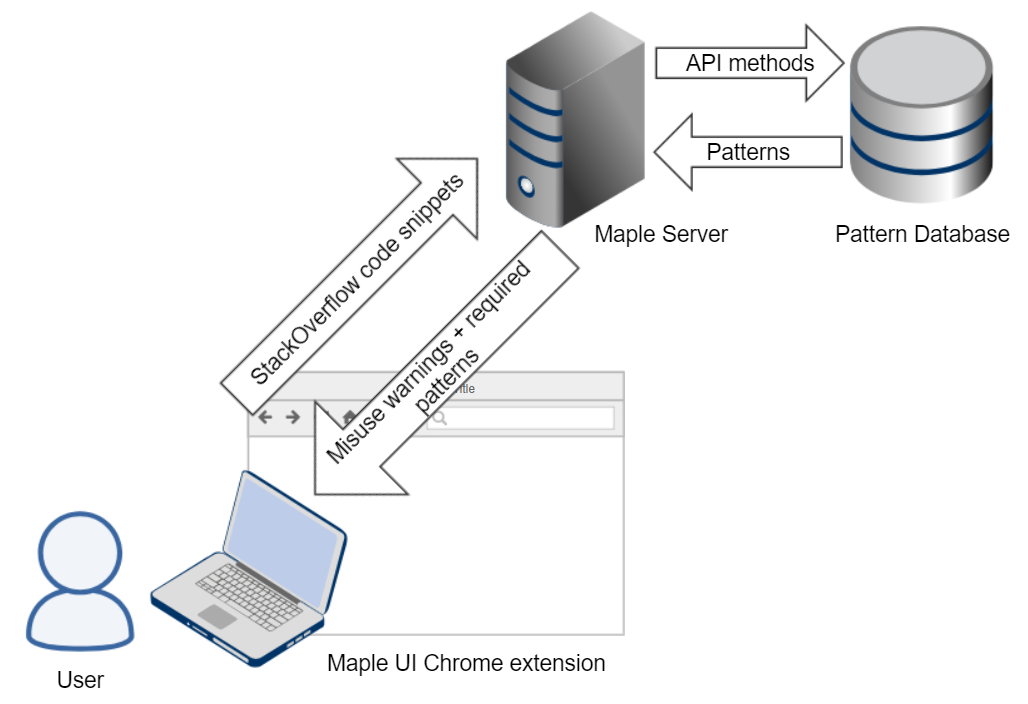
\includegraphics[width=0.48\textwidth]{mapleUIsystemflow.PNG}
\vspace{.1in}
\caption{An overview of {\soa}'s architecture\todo{Maybe we can add more details to this diagram. For example, we can show what we do in the server, and the interaction between the server and Boa's GitHub database.}}
\label{fig:arch}
\end{figure}

% Solution
To assess online code examples, this paper presents {\soa}, an interactive approach that augments Stack Overflow with code idioms learned from GitHub and alerts programmers about the potential violations in a code example. {\soa} leverges a scalable API usage mining technique to learn three types of API-related idioms---temporal ordering, guard conditions, and exception handling of API calls---from over 7 million GitHub projects. Our insight is that commonly practiced idioms in massive code corpora may represent a desirable pattern that a programmer can use to trust and enhance code examples on Stack Overflow. 

Given an SO example, {\soa} first extracts the sequence of API calls with corresponding control constructs and guard conditions. {\soa} then contrasts the sequence with commonly practiced idioms in GitHub and highlights code regions that violate the idioms. To help users better understand the violations, {\soa} further generates descriptive warning messages and also contextualizes a violated idiom by synthesizing a fixed example. Mining code idioms to detect API usage violations often suffers from reporting false alarms, since mined idioms may not be inclusive and fit all use scenarios of an API~\cite{liang2016antminer}. To mitigate this issue, {\soa} allows users to upvote or downvote a violation based on its applicability and usefulness to an SO example. {\soa} filters a code idiom when multiple users flag it as unhelpful to assess an example. To help developers build confidence on a code idiom, {\soa} shows how many GitHub developers also follow the idiom as well as how many other users like or dislike this idiom.

A user of {\soa} would benefit from the addition of quantitative examples from compiled GitHub resources to the code examples she encounters on Stack Overflow. This will not only combat programming issues stemming from the use of incomplete or unreliable SO code examples, but will also be an aid for users learning a new API. By enhancing examples already found in Stack Overflow, a user can trust that she will learn common and reliable usage patterns for a given API.
%A user of this tool would benefit from not needing to cross-reference multiple sites for proper API usage reference, and will be able to continue using Stack Overflow to learn APIs with the added advantage of seeing which usage patterns a post may have left out of its explanation. This could result in more complete, reliable code with minimal added time or effort on the part of the programmer.\todo{The description here does not sound very appealing. Can you rework this paragraph?} 

This paper's main contribution is to describe the features of {\soa} from a user's perspective. In order to give programmers access to {\soa}, the front-end of {\soa} is implemented as a Chrome extension that users can easily download and install.\todo{add a url to download our tool} The detailed algorithm and study are described in our separate technical report.\todo{cite our API misuse study}

%input{fig_motiExample}
%\input{fig_UI}
